%!TEX root = ../thesis.tex
\appendix
\chapter{The Bullard-Gellman Formalism}
\label{chap:appendix1}
One important way of understanding how dynamos operate is called the Bullard-Gellman formalism  \citep{bullard1954}. This simplified framework was developed to study how interactions between fluid motion and seed magnetic fields can generate new magnetic fields. While a detailed derivation of this formalism is outside the scope of this work (see \citet{bullard1954}) we will introduce the basic derivation here, which will allow us to interpret the results of chapter \ref{chap:superearth}.

The Bullard-Gellman formalism begins with the assumption of an incompressible fluid in a sphere of non-dimensional radius 1 and seeks to find solutions to the equations
\begin{align}
\frac{\partial \mbf{B}}{\partial t}&=\nabla\times\left(\mbf{u}\times\mbf{B}\right)+\eta\nabla^{2}\mbf{B} & \textrm{for } r<1
\end{align}
of the form
\begin{equation}
\mbf{B}\left(\mbf{r},t\right)=\mbf{B}\left(\mbf{r}\right)e^{\lambda t}.
\end{equation}
Substituting this into this into the magnetic induction equation means we seek to find solutions to 
\begin{equation}
\left(\lambda-\nabla^{2}\right)\mbf{B}=\nabla\times\left(\mbf{u}\times\mbf{B}\right)\label{eq:bgmie}.
\end{equation}
Using the Toroidal-Poloidal expansion (equation \ref{eq:toroidalpoloidal}\footnote{This expansion differs in form from the expansion we saw in equation \ref{eq:laplaceexpansion}. In this case $A_{l}^{m}$ can be complex which will make the subsequent expressions simpler.}) along with the spherical harmonic expansion
\begin{equation}
A=\sum_{l=1}^{\infty}\sum_{m=0}^{l}A_{l}^{m}Y_{l}^{m}\left(\theta,\phi\right)
\end{equation}
on the magnetic field and velocity field to give
\begin{align}
\mbf{B}=\mbf{B}_{T}+\mbf{B}_{P}=\sum_{L=1}^{\infty}\sum_{m=0}^{L} \left(\mbf{T}_{l}^{m}+\mbf{P}_{l}^{m}\right) \\
\mbf{u}=\mbf{u}_{T}+\mbf{u}_{P}=\sum_{L=1}^{\infty}\sum_{m=0}^{L} \left(\mbf{t}_{l}^{m}+\mbf{p}_{l}^{m}\right).
\end{align}
Here we have denoted a single component of the magnetic field in capital letters (e.g. $\mbf{T}_{l}^{m}$) and a single component of the velocity field in lower case letters (e.g. $\mbf{t}_{l}^{m}$). Following the definition of equation \ref{eq:toroidalpoloidal} we can write
\begin{align}
\mbf{T}_l^m &= \nabla \times \left[T_l^m\left(r\right) Y_l^m \left(\theta, \phi\right) \hat{r}\right] \label{eq:Texpansion}\\ 
\mbf{P}_l^m &= \nabla \times \nabla \times \left[P_l^m\left(r\right) Y_l^m \left(\theta, \phi\right) \hat{r}\right]\label{eq:Pexpansion} \\
\mbf{t}_l^m &= \nabla \times \left[t_l^m\left(r\right) Y_l^m \left(\theta, \phi\right)\hat{r}\right] \label{eq:texpansion}\\
\mbf{p}_l^m &= \nabla \times \nabla \times \left[p_l^m\left(r\right) Y_l^m \left(\theta, \phi\right) \hat{r}\right].\label{eq:pexpansion}
\end{align}
If we substitute equations \ref{eq:Texpansion}-\ref{eq:pexpansion} into \ref{eq:bgmie} we get
\begin{equation}
 (\lambda-\nabla^2) \left[\sum_1 \left(\mbf{T}_{l_1}^{m_1} + \mbf{P}_{l_1}^{m_1}\right)\right]
  = \nabla \times \left[\sum_2 \left(\mbf{t}_{l_2}^{m_2} +
  \mbf{p}_{l_2}^{m_2}\right)\right] \times \left[\sum_3 \left(\mbf{T}_{l_3}^{m_3} +
  \mbf{P}_{l_3}^{m_3}\right)\right] \label{eq:bgexpand1}
\end{equation}
where the subscripts under the sums indicate that we sum over the $l$ and $m$ of that index. This expression gives a sum over resultant magnetic field components (subscript $1$) produced by all velocity modes (subscript $2$) acting on all magnetic field modes (subscript $3$). In order to get interpretable predictions, we would like to know the growth rate of one mode (one $l_1$, $m_1$ combination) due to specific velocity and magnetic field modes. To get this, we will take the inner product of equation \ref{eq:bgexpand1} with a single toroidal or poloidal mode which are defined as:
\begin{align}
\left[\nabla\times\left(Y_{l_1}^{m_1}\right)\hat{r}\right]^{*}\\
\left[\nabla\times\nabla\times\left(Y_{l_1}^{m_1}\right)\hat{r}\right]^{*}
\end{align}
respectively, giving
\begin{multline}
\oint_S \left[\nabla \times (Y_{l_1}^{m_1}(\theta,\phi)\hat{r})\right]^* \cdot (\lambda-\nabla^2)  \left[\sum_1
      \left(\mbf{T}_{l_1}^{m_1} + \mbf{P}_{l_1}^{m_1}\right)\right] dS = \\
 \oint_S \left[\nabla \times(Y_{l_1}^{m_1}(\theta,\phi)\hat{r})\right]^* \cdot \nabla \times \left[\sum_2 \left(\mbf{t}_{l_2}^{m_2} +
  \mbf{p}_{l_2}^{m_2}\right)\right] \times \left[\sum_3
\left(\mbf{T}_{l_3}^{m_3} + \mbf{P}_{l_3}^{m_3}\right)\right] dS \label{eq:bgtorexpand2}
\end{multline}
and
\begin{multline}
\oint_S \left[\nabla \times \nabla \times (Y_{l_1}^{m_1}(\theta,\phi)\hat{r})\right]^* \cdot (\lambda-\nabla^2)  \left[\sum_1
      \left(\mbf{T}_{l_1}^{m_1} + \mbf{P}_{l_1}^{m_1}\right)\right] dS = \\
 \oint_S \left[\nabla \times \nabla \times(Y_{l_1}^{m_1}(\theta,\phi)\hat{r})\right]^* \cdot \nabla \times \left[\sum_2 \left(\mbf{t}_{l_2}^{m_2} +
  \mbf{p}_{l_2}^{m_2}\right)\right] \times \left[\sum_3
\left(\mbf{T}_{l_3}^{m_3} + \mbf{P}_{l_3}^{m_3}\right)\right] dS.\label{eq:bgpolexpand2}
\end{multline}
Using the orthonormality properties of our toroidal and poloidal fields, as well as the identity
\begin{equation}
\nabla^{2}Y_{l}^{m}=\left[\frac{1}{r^2}\frac{\partial}{\partial r}\left(r^{2}\frac{\partial}{\partial r}\right)-\frac{l\left(l+1\right)}{r^2}\right]Y_{l}^{m}
\end{equation}
i.e. that spherical harmonics are eigenvectors of the angular part of the Laplacian, and the following identities concerning our toroidal and poloidal fields:
\begin{align}
\mbf{T}_{l}^{m}&=\nabla\times\left(T_{l}^{m}\left(r\right)Y_{l}^{m}\left(\theta,\phi\right)\hat{r}\right)=T_{l}^{m}\left(r\right)\nabla\times\left(Y_{l}^{m}\left(\theta,\phi\right)\hat{r}\right)\\
\mbf{P}_{l}^{m}&=\nabla\times\nabla\times\left(P_{l}^{m}\left(r\right)Y_{l}^{m}\left(\theta,\phi\right)\hat{r}\right)=P_{l}^{m}\left(r\right)\nabla\times\left(Y_{l}^{m}\left(\theta,\phi\right)\hat{r}\right)\\
\mbf{t}_{l}^{m}&=\nabla\times\left(t_{l}^{m}\left(r\right)Y_{l}^{m}\left(\theta,\phi\right)\hat{r}\right)=t_{l}^{m}\left(r\right)\nabla\times\nabla\times\left(Y_{l}^{m}\left(\theta,\phi\right)\hat{r}\right)\\
\mbf{p}_{l}^{m}&=\nabla\times\nabla\times\left(p_{l}^{m}\left(r\right)Y_{l}^{m}\left(\theta,\phi\right)\hat{r}\right)=p_{l}^{m}\left(r\right)\nabla\times\nabla\times\left(Y_{l}^{m}\left(\theta,\phi\right)\hat{r}\right)
\end{align}
we can write equations \ref{eq:bgtorexpand2} and \ref{eq:bgpolexpand2} as 
\begin{multline}
\left(\lambda-\nabla^{2}\right)T_{l_1}^{m_1}\left(r\right)=\sum_{1}\sum_{2}
%
t_{l_2}^{m_2} T_{l_3}^{m_3} \oint_S \left[\nabla \times (Y_{l_1}^{m_1}(\theta,\phi)\hat{r})\right]^* \cdot 
\left[\nabla\times\left\{ \left(\nabla\times Y_{l_2}^{m_2}\hat{r}\right)\times \left(\nabla\times Y_{l_3}^{m_3}\hat{r}\right)   \right\}\right]  \\
+
p_{l_2}^{m_2} T_{l_3}^{m_3} \oint_S  \left[\nabla \times (Y_{l_1}^{m_1}(\theta,\phi)\hat{r})\right]^* \cdot
\left[\nabla\times\left\{ \left(\nabla\times\nabla\times Y_{l_2}^{m_2}\hat{r}\right)\times \left(\nabla\times Y_{l_3}^{m_3}\hat{r}\right)   \right\}\right]\\
+
t_{l_2}^{m_2} P_{l_3}^{m_3} \oint_S  \left[\nabla \times (Y_{l_1}^{m_1}(\theta,\phi)\hat{r})\right]^* \cdot 
\left[\nabla\times\left\{ \left(\nabla\times Y_{l_2}^{m_2}\hat{r}\right)\times \left(\nabla\times\nabla\times Y_{l_3}^{m_3}\hat{r}\right)   \right\}\right]  \\
+
p_{l_2}^{m_2} P_{l_3}^{m_3} \oint_S  \left[\nabla \times (Y_{l_1}^{m_1}(\theta,\phi)\hat{r})\right]^* \cdot
\left[\nabla\times\left\{ \left(\nabla\times\nabla\times Y_{l_2}^{m_2}\hat{r}\right)\times \left(\nabla\times\nabla\times Y_{l_3}^{m_3}\hat{r}\right)   \right\}\right]
\label{eq:bgtorexpand3}
\end{multline}
and 
\begin{multline}
\left(\lambda-\nabla^{2}\right)P_{l_1}^{m_1}\left(r\right)=\sum_{1}\sum_{2}
%
 t_{l_2}^{m_2} T_{l_3}^{m_3} \oint_S\left[\nabla\times \nabla \times (Y_{l_1}^{m_1}(\theta,\phi)\hat{r})\right]^* \cdot 
\left[\nabla\times\left\{ \left(\nabla\times Y_{l_2}^{m_2}\hat{r}\right)\times \left(\nabla\times Y_{l_3}^{m_3}\hat{r}\right)   \right\}\right]  \\
+
p_{l_2}^{m_2} T_{l_3}^{m_3} \oint_S  \left[\nabla\times\nabla \times (Y_{l_1}^{m_1}(\theta,\phi)\hat{r})\right]^* \cdot
\left[\nabla\times\left\{ \left(\nabla\times\nabla\times Y_{l_2}^{m_2}\hat{r}\right)\times \left(\nabla\times Y_{l_3}^{m_3}\hat{r}\right)   \right\}\right]\\
+
t_{l_2}^{m_2} P_{l_3}^{m_3} \oint_S  \left[\nabla\times\nabla \times (Y_{l_1}^{m_1}(\theta,\phi)\hat{r})\right]^* \cdot 
\left[\nabla\times\left\{ \left(\nabla\times Y_{l_2}^{m_2}\hat{r}\right)\times \left(\nabla\times\nabla\times Y_{l_3}^{m_3}\hat{r}\right)   \right\}\right]  \\
+
p_{l_2}^{m_2} P_{l_3}^{m_3} \oint_S \left[\nabla\times\nabla \times (Y_{l_1}^{m_1}(\theta,\phi)\hat{r})\right]^* \cdot
\left[\nabla\times\left\{ \left(\nabla\times\nabla\times Y_{l_2}^{m_2}\hat{r}\right)\times \left(\nabla\times\nabla\times Y_{l_3}^{m_3}\hat{r}\right)   \right\}\right].
\label{eq:bgpolexpand3}
\end{multline}
All of the integrals in equations \ref{eq:bgtorexpand3} and \ref{eq:bgpolexpand3} can be represented as an integral of the form
\begin{equation}
G = \oint_S Y_{l_1}^{m_1*}Y_{l_2}^{m_2}Y_{l_3}^{m_3} dS \label{eq:adamsgaunt}
\end{equation}
or
\begin{equation}
L = \oint_S Y_{l_1}^{m_1*}\left(\frac{\partial
        Y_{l_2}^{m_2}}{\partial \theta}\frac{\partial
        Y_{l_3}^{m_3}}{\partial \phi} - \frac{\partial
        Y_{l_2}^{m_2}}{\partial \phi}\frac{\partial
        Y_{l_3}^{m_3}}{\partial \theta}\right) dS. \label{eq:elsasser}
\end{equation}
Integrals of the form in equation \ref{eq:adamsgaunt} are known as Adams-Gaunt integrals, and integrals of the form in equation \ref{eq:elsasser} are known as Elsasser integrals. For simplicity, and historical reasons we will introduce some notation to simplify equations \ref{eq:bgtorexpand3} and \ref{eq:bgpolexpand3}. We will say the spherical harmonic index of the magnetic field being created is $\gamma$, the velocity field will have index $\alpha$ and the seed magnetic field will have index $\beta$. Furthermore, we will represent terms involving a poloidal field (e.g. $\nabla\times\nabla\times Y_{l_2}^{m_2}\hat{r}$) as $P$ and terms representing a toroidal field (e.g. $\nabla\times Y_{l_2}^{m_2}\hat{r}$) as $T$. For example, we could then represent the integral
\begin{equation}
p_{l_2}^{m_2} P_{l_3}^{m_3} \oint_S \left[\nabla\times\nabla \times (Y_{l_1}^{m_1}(\theta,\phi)\hat{r})\right]^* \cdot
\left[\nabla\times\left\{ \left(\nabla\times\nabla\times Y_{l_2}^{m_2}\hat{r}\right)\times \left(\nabla\times\nabla\times Y_{l_3}^{m_3}\hat{r}\right)   \right\}\right]
\end{equation}
as $P_{\alpha}P_{\beta}P_{\gamma}$. If we wish to refer to the order of the spherical harmonic we will refer to it as $m_\gamma$, $m_\alpha$, or $m_\beta$. Under this notation equations  \ref{eq:bgtorexpand3} and \ref{eq:bgpolexpand3} can be represented as 
\begin{equation}
\left(\lambda-\nabla^{2}\right)T_{\gamma}\left(r\right)=\sum_{\alpha,\beta}\left(T_\alpha T_\beta T_\gamma +P_\alpha T_\beta T_\gamma+T_\alpha P_\beta T_\gamma+P_\alpha P_\beta T_\gamma\right)\label{eq:bgtorexpand4}
\end{equation}
and 
\begin{equation}
\left(\lambda-\nabla^{2}\right)P_{\gamma}\left(r\right)=\sum_{\alpha,\beta}\left(T_\alpha T_\beta P_\gamma +P_\alpha T_\beta P_\gamma+T_\alpha P_\beta P_\gamma+P_\alpha P_\beta P_\gamma\right).\label{eq:bgpolexpand4}
\end{equation}
The Adams-Gaunt types integral are 
\begin{align}
P_\alpha P_\beta P_\gamma \\
T_\alpha P_\beta T_\gamma \\
P_\alpha T_\beta T_\gamma,
\end{align}
the Elsasser type integrals are
\begin{align}
T_\alpha P_\beta P_\gamma \\
P_\alpha T_\beta P_\gamma \\
P_\alpha P_\beta T_\gamma \\
T_\alpha T_\beta T_\gamma
\end{align}
while integrals of the form $T_\alpha T_\beta P_\gamma$ are always zero.

Equations \ref{eq:bgtorexpand4} and \ref{eq:bgpolexpand4} have a straightforward interpretation, in order for a given magnetic field mode ($\gamma$) to grow, the right hand sides of these equations must be greater than zero. This requires the evaluation of the integrals in these equations. The integrals in  \ref{eq:bgtorexpand4} and \ref{eq:bgpolexpand4} are zero in many cases, the instances where they are \emph{not} are defined by selection rules. For the Adams-Gaunt type, the integral is zero unless:
\begin{itemize}
\item $\alpha+\beta+\gamma$ is even.
\item $\alpha, \beta, \gamma$ can form the sides of a triangle. This is equivalent to satisfying the triangle inequality: $\left|\alpha-\beta\right|<\gamma<\alpha+\beta$.
\item One or more of $m_\alpha \pm m_\beta \pm m_\gamma$ is zero.
\item Either three or one of the harmonics has a $\cos\left(m\phi\right)$ term, with $m=0$ counting as a $\cos\left(m\phi\right)$.
\end{itemize}
Elsasser integrals are zero unless:
\begin{itemize}
\item $\alpha+\beta+\gamma$ is odd.
\item $\alpha, \beta, \gamma$ can form the sides of a triangle. This is equivalent to satisfying the triangle inequality: $\left|\alpha-\beta\right|<\gamma<\alpha+\beta$.
\item One or more of $m_\alpha \pm m_\beta \pm m_\gamma$ is zero.
\item Either two or none of the harmonics has a $\cos\left(m\phi\right)$ term, with $m=0$ counting as a $\cos\left(m\phi\right)$.
\item No two harmonics are identical.
\end{itemize}
It is important to note that the only way a magnetic field can be maintained in this framework is if there is a way for magnetic energy induced from a mode ($\beta$) to eventually be fed back into that mode. If this does not take place, the energy supplied by $\mbf{u}$ in mode $\alpha$ will be dissipated over infinitely many magnetic field modes and diffused away at small scale.

A useful tool to visualise how magnetic fields are generated in this framework is an \emph{interaction diagram}. In an interaction diagram the dynamo process is represented as a directed graph with vertices forming magnetic field nodes (which can be induced or seed fields) and vertices representing the velocity field modes. 

For example, one finite interaction diagram occurs when $P_1^0$ ($\beta=1$, $m_\beta=0$) is acted on by $T_1^0$ ($\alpha=1$, $m_\alpha=0$) to produce $T_2^0$ ($\gamma=2$, $m_\gamma=0$). This would be represented in an interaction diagram as figure \ref{fig:interaction-differentialrotation}.
\begin{figure}
	\centering
	\noindent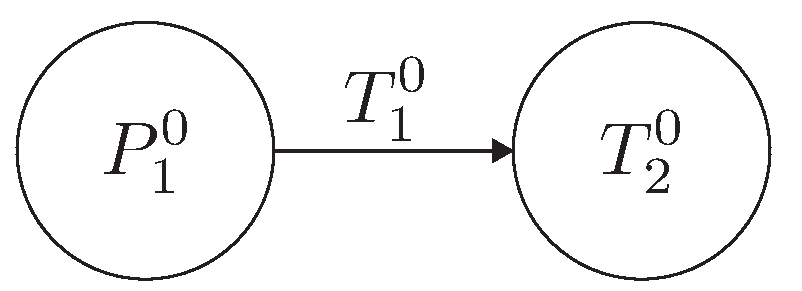
\includegraphics[width=.45\linewidth]{Appendix1/figures/interaction-differentialrotation.pdf}
	\caption{A simple closed interaction diagram. Here a magnetic field $P_1^0$ is acted on by velocity field $T_1^0$ to produce magnetic field $T_2^0$}
	\label{fig:interaction-differentialrotation}
\end{figure}
Another closed interaction diagram is shown in figure \ref{interaction-complicated.pdf}, this is considerably more complicated than figure \ref{fig:interaction-differentialrotation}.
\begin{figure}
	\centering
	\noindent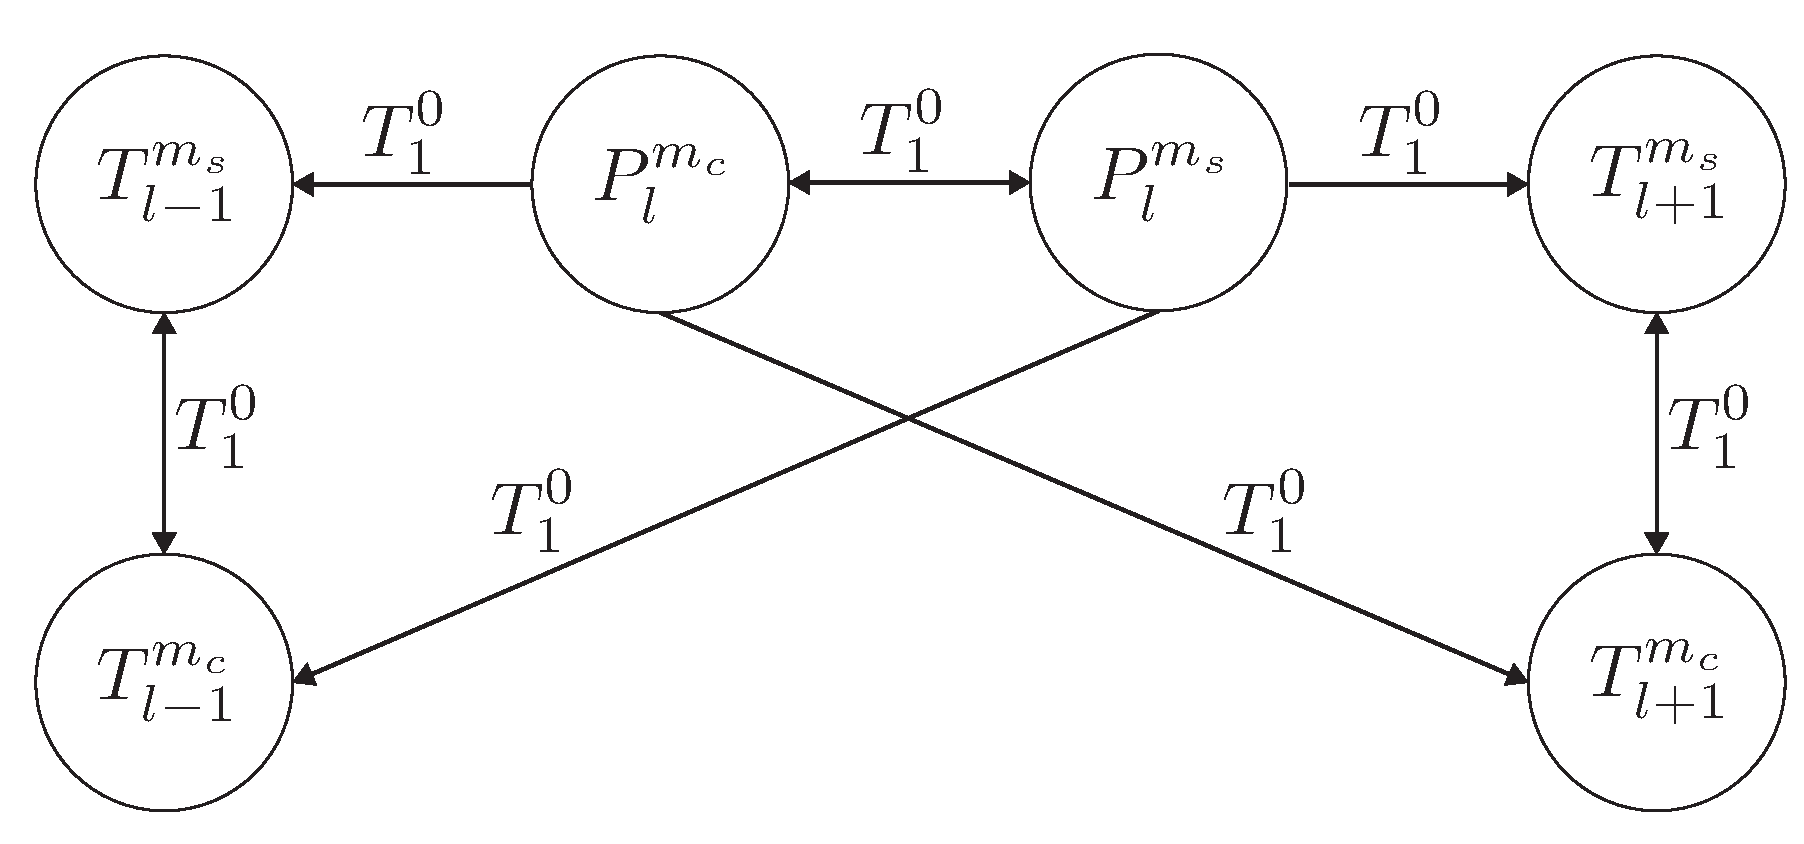
\includegraphics[width=\linewidth]{Appendix1/figures/interaction-complicated.pdf}
	\caption{A more complicated closed interaction diagram. Here a magnetic field $P_1^0$ is acted on by velocity field $T_1^0$ to produce magnetic field $T_2^0$}
	\label{interaction-complicated.pdf}
\end{figure}
Neither of these interaction diagrams represent self-sustaining dynamo as the velocity field is in both is purely toroidal. A purely toroidal velocity field contains no radial component of velocity. This is important because \citet{busse1975} showed that a radial component of the velocity field is a necessary condition for a self sustaining dynamo. 

We have not considered the radial dependence of equations \ref{eq:bgtorexpand4} and \ref{eq:bgpolexpand4} or the boundary conditions associated with them. These details complicate matters somewhat, however an evaluation of the angular terms provides us with a necessary condition for dynamo action which sufficient for the argument we make in chapter \ref{chap:superearth}.
